%%LectureNote01 pre
%\begin{flushright}
%   2024年10月7日
%   
%   九大・数理 大津幸男
%\end{flushright}
%
%\begin{center}
%   \large{微分幾何学大意・数学特論4\small{
%   \href{https://creativecommons.org/licenses/by-nc-nd/4.0/}{\ccbyncnd}}
%   \par ---直交群とその有限部分群 1---}
%\end{center}
%
%\begin{PP}
%   ユークリッド幾何から派生した幾何学・群論・関数論を解説し，
%   現代的な微分幾何への橋渡しを行う．更にプログラミングとアート
%   との関連を探る．
%\end{PP}

\chapter{$2$, $3$次元直交群の有限部分群の分類}
\section{$2$次元直交群の有限部分群}
\subsection{$\mathbf R^2$の線形合同変換の例}
ユークリッド平面$\mathbf R^2$の全ての点$(x,y)$に$\mathbf R^2$の別の点$(x',y')$を対応させる対応を（$\mathbf R^2$の）\term[]{変換}という．
平面$\mathbf R^2$の点$(x,y)$と複素平面$\mathbf C$の点$x+iy$を同一視する．（高校でやったように）原点を中心にした\term[]{回転}(rotation)は$\cos\theta+i\sin\theta$を掛けることに対応するので
\[
     (\cos\theta+i\sin\theta)(x+iy)
     =x\cos\theta-y\sin\theta+i(x\sin\theta+y\cos\theta)
\]
つまり，
\[
     \begin{pmatrix}
          x\cos\theta-y\sin\theta\\
          x\sin\theta+y\cos\theta\\
     \end{pmatrix}
     =
     \begin{pmatrix}
          \cos \theta &-\sin \theta\\
          \sin \theta& \cos \theta\\
     \end{pmatrix}
     \begin{pmatrix}
          x\\
          y\\
     \end{pmatrix}
     =S_\theta\mathbf x
\]
と行列の積で表すことが出来る，ここで，
\[
     S_\theta=
     \begin{pmatrix}
          \cos \theta &-\sin \theta\\
          \sin \theta& \cos \theta\\
     \end{pmatrix},\quad
     \mathbf x
     =
     \begin{pmatrix}
          x\\
          y\\
     \end{pmatrix}.
\]
このように行列の積で表される変換を\term[]{線形変換}という．
また，距離を保つ変換を\term[]{合同変換}という，回転は合同変換の一つである（距離については次の節で詳しく述べる）．
また，
\begin{equation}\label{rel1}
     S_\theta S_\tau=S_{\theta+\tau},\quad S_0=E
\end{equation}
特に
\[
     S_{-\theta}S_\theta=E,\quad S_{\theta}^{-1}
     =S_{-\theta}={}^tS_{\theta}
\]
ただし，$E$は単位行列$(\delta_{ij})$．
\begin{figure}[htb]
   \centering
   \begin{minipage}{0.4\columnwidth}
      \centering
        \includegraphics{~/Documents/GitHub/bEuclideanGeo/ch1/images/figureGroup.1}
        \caption{原点での回転}\label{}
   \end{minipage} 
   \begin{minipage}{0.4\columnwidth}
      \centering
        \includegraphics{~/Documents/GitHub/bEuclideanGeo/ch1/images/figureGroup.2}
        \caption{$x$軸での鏡映}\label{}
   \end{minipage} 
\end{figure}

（複素共役$z\mapsto \bar z$に対応する）$x$軸での\term[]{鏡映（折り返し）}(refrection)は$(x,y)$に$(x,-y)$を対応させることなので，
\[
      \begin{pmatrix}
          x\\
          -y\\
     \end{pmatrix}
     =
     \begin{pmatrix}
          1&0\\
          0&-1\\
     \end{pmatrix}
     \begin{pmatrix}
          x\\
          y\\
     \end{pmatrix}
\]
と線形変換で表すことが出来る，これも合同変換でもある．一般に，
直線$\ell: -x\sin\theta+y\cos\theta=0$についての鏡映の，
行列の積を使った表現を求める：
$\ell$の単位法線ベクトルは
\[
     \mathbf e
     =\begin{pmatrix}
          -\sin\theta\\
          \cos\theta\\
     \end{pmatrix}
\]
であるので$\mathbf x$との
内積は$ (\mathbf e,\mathbf x)=-x\sin\theta+y\cos\theta$．
$\mathbf x$を$\mathbf e$方向の成分とその直交成分にわけると
\[
     \mathbf x= (\mathbf e,\mathbf x)\,\mathbf e
     +\{\mathbf x- (\mathbf e,\mathbf x)\,\mathbf e\}.
\]
\begin{figure}[htb]
   \centering
   \begin{minipage}{0.4\columnwidth}
        \centering
        \includegraphics{~/Documents/GitHub/bEuclideanGeo/ch1/images/figureGroup.3}
        \caption{直線$\ell$での鏡映}\label{}\end{minipage} 
   \begin{minipage}{0.4\columnwidth}
      \centering
      \includegraphics{~/Documents/GitHub/bEuclideanGeo/ch1/images/figureGroup.4}
      \caption{鏡映と鏡映の合成}\label{compRefs}
   \end{minipage} 
\end{figure}
$ (\mathbf e,\mathbf x)\,\mathbf e$ は$\mathbf x$の$\mathbf e$成分，
$\mathbf x- (\mathbf e,\mathbf x)\, \mathbf e$ は直交成分．
$\ell$についての鏡映は（図3）
\[
     \{\mathbf x- (\mathbf e,\mathbf x)\,\mathbf e\}
          - (\mathbf e,\mathbf x)\,\mathbf e
     =\mathbf x-2 (\mathbf e,\mathbf x)\,\mathbf e.
\]
これをベクトルの成分で計算すると
\[
\begin{split}
     \mathbf x-2 (\mathbf e,\mathbf x)\,\mathbf e
     &=
     \begin{pmatrix}
          x\\
          y\\
     \end{pmatrix}
     -2(-x\sin\theta+y\cos\theta)
     \begin{pmatrix}
          -\sin\theta\\
          \cos\theta\\
     \end{pmatrix}\\
     &=
     \begin{pmatrix}
          x(1-2\sin^2\theta)+2y\cos\theta\sin\theta\\
          2x\sin \theta \cos\theta+y(1-2\cos^2\theta)\\
     \end{pmatrix}\\
     &=\begin{pmatrix}
          \cos 2\theta &\sin 2\theta\\
          \sin 2\theta&-\cos 2\theta\\
     \end{pmatrix}
     \begin{pmatrix}
          x\\
          y\\
     \end{pmatrix}
     =R_{\theta}\mathbf x,
\end{split}
\]
ここで
\[
     R_{\theta}
     =
     \begin{pmatrix}
          \cos 2\theta &\sin 2\theta\\
          \sin 2\theta&-\cos 2\theta\\
     \end{pmatrix}.
\]
直線$\ell$を鏡映の軸とも言う．

同じ直線についての鏡映を2回続けると元に戻るので
\begin{equation}\label{rel2}
     R_{\theta}^2=R_{\theta}R_{\theta}=E,
     \quad\text{言い換えると}\quad 
     R_{\theta}^{-1} =R_{\theta}={}^tR_{\theta}.
\end{equation}
$\mathbf 0$を通る直線に沿っての二つの鏡映の合成は$\mathbf 0$についての回転になる：行列の積で表すと
\begin{equation}\label{rel3}
     R_{\theta}R_{\tau}=S_{2(\theta-\tau)}
     \quad\text{よって}\quad
     R_{\theta}=S_{2(\theta-\tau)}R_{\tau}.
\end{equation}
これは初等幾何学を使うことでわかる（図~\ref{compRefs}）が，単に行列の積を計算することでもわかる．
%アプリ./reflections/p5の実行
%アプリ./reflections/p5の実行
%アプリ./reflections/p5の実行

%
%問　回転と回転の合成は回転なので
%\[
%     S_\theta S_\tau=S_{\theta+\tau}
%\]
%が成り立つ．これを行列の積を計算することで確かめよ．
%
%
%問　二つの直線が交わらないとき，つまり，平行なとき，これらの直線に沿っての二つの鏡映の合成は何になるか？
%

\subsection{一般の直交変換群}
$n$を自然数とし$n$次元ユークリッド空間$\mathbf R^n$を考える．
\[
     (\mathbf u,\mathbf v)={}^t\mathbf u\mathbf v
     =u_1v_1+u_2v_2+\cdots+u_nv_n\in \mathbf R
     \quad
     \mathbf u
      =\begin{pmatrix}
              u_1\\u_2\\\vdots\\u_n
     \end{pmatrix},
     \mathbf v
      =\begin{pmatrix}
              v_1\\v_2\\\vdots\\v_n
     \end{pmatrix}
     \in \mathbf R^n
\]
と置き，$\mathbf R^n$の\term[]{標準内積}という．
${}^tA=(b_{ij})$は$A=(a_{ij})$の転置行列，つまり，$b_{ij}=a_{ji}$．
$(\mathbf u,\mathbf u)\ge 0$なので
\[
     \|\mathbf u\| 
     = 
     \sqrt{(\mathbf u,\mathbf u)}
     \ge 0
\]
と置き，\term[]{ノルム}（\term[]{長さ}）という．

$T:\mathbf R^n\to \mathbf R^n$が\term[]{直交変換}とは
\begin{equation}\label{orthogonalTransform}
     (T(\mathbf u),T(\mathbf v))
     =
     (\mathbf u,\mathbf v)\quad
     \mathbf u,\mathbf v\in \mathbf R^n
\end{equation}
が成り立つことである．この定義から直交変換はノルムを保存することが分かる：
\begin{equation}\label{preserveNorm}
     \|T(\mathbf u)\| = \|\mathbf u\| 
\end{equation}
逆にこれが成り立てば直交変換になることも簡単に分かる．したがって
直交変換は合同線形変換である．

$n$次正方行列$A$が\term[]{直交行列}とは
\[
     {}^tAA=E
\]
が成り立つことであり，これは
\[
     A^{-1}={}^tA
\]と同値である．
したがって，回転$S_\theta$や鏡映$R_{\theta}$は直交行列である．

$n$次正方行列$A$に対して$T_A(\mathbf x)=A\mathbf x$で線形変換を定義すると
\[
     T_A\text{ が直交変換}
     \Leftrightarrow 
     A\text{ が直交行列}
\]
$\Leftarrow)$は
\[
\begin{split}
     (T_A(\mathbf u),T_A(\mathbf v))
     &=
     (A\mathbf u,A\mathbf v)
     =
     {}^t(A\mathbf u)A\mathbf v
     =
     {}^t\mathbf u{}^tAA\mathbf v\\
     &
     =
     {}^t\mathbf u({}^tAA)\mathbf v
     =
     {}^t\mathbf uE\mathbf v
     =
     {}^t\mathbf u\mathbf v
     =
     (\mathbf u,\mathbf v)
\end{split}
\]
よりわかる．

$\Rightarrow)$は，
\[
     \mathbf e_1=
     \begin{pmatrix}
              1\\0\\0\\\vdots\\0
     \end{pmatrix},
     \mathbf e_2=
     \begin{pmatrix}
              0\\1\\0\\\vdots\\0
     \end{pmatrix},     
     \cdots,
     \mathbf e_n=
     \begin{pmatrix}
              0\\0\\\vdots\\0\\1
     \end{pmatrix}
\]
を$\mathbf R^n$の標準基とし，
\eqref{orthogonalTransform}の式で
$\mathbf u=\mathbf e_i$, $\mathbf v=\mathbf e_j$ ととると
${}^tAA$と$E$の$(i,j)$成分が一致することが分かるので示せた．
\emptyline

集合$G$が\term[]{群}であるとは任意の$a$, $b\in G$に対して積$ab\in G$が定まり，次の三条件を満たすことである：
\[
     (ab)c = a(bc)\quad \forall a, b, c\in G
\]
を満たす．
単位元$e\in G$が存在し，
\[
     ea=ae=a\quad \forall a\in G
\]
を満たす．また任意の$a\in G$に対して逆元$a^{-1}$が存在して
\[
     aa^{-1}= a^{-1}a = e
\]
を満たす．単位元や逆元の一意性は直ぐに分かる．
\emptyline

$H\subset G$が\term[]{部分群}とは$H$が$G$の積に関して群となることである．これは
\[
     a,b\in H\Rightarrow ab\in H\quad\text{かつ}\quad 
     a\in H\Rightarrow a^{-1}\in H
\]
を満たすことと同値である．
\emptyline

正方行列$A$の行列式を$|A| $あるいは$\det A$と表すと
\[
     |AB|=|A||B|
\]
で，$|A|\neq0$が$A$が正則であることと同値なので
\[
     \GL(n;\mathbf R)=\{A\mid n\text{次正則行列} \}
\]
は
群になる．

直交行列$A$については
$1=|E|=|{}^tA||A|=|A|^2$より$|A|=\pm 1$．
\[
     \Ot(n)=\{A\in \GL(n;\mathbf R)\mid \text{直交行列}\},\quad
     \SO(n)=\{A\in \Ot(n)\mid |A|=1\}
\]
と置くと，
$A$, $B\in \Ot(n)$に対して
\[
     {}^t(AB)AB={}^tB{}^tA AB ={}^tBEB={}^tBB=E
\]
となり，
\[
     A^{-1}={}^tA \quad\text{より}\quad (A^{-1})^{-1}
     =A
     ={}^t({}^tA)={}^t(A^{-1})
\]
なるので$\Ot(n)$は$\GL(n;\mathbf R)$の部分群になる．$A$, $B\in \SO(n)$に対して
\[
     |AB|=|A||B| =1\times 1=1,\quad
     |A^{-1}| =|{}^tA| = |A| =1
\]
となるので$\SO(n)$も群で$\Ot(n)$の部分群である．
\emptyline

$\GL(n;\mathbf R)$を$n$次元\term[]{一般線形群}(General linear group)，
$\Ot(n)$を$n$次元\term[]{直交群}(Orthogonal group)，$\SO(n)$を$n$次元\term[]{特殊直交群}(Special Orthogonal group)という．

%\emptyline
%
%群が多様体で，積を与える写像と逆を与える写像が微分可能になっているとき
%\term[]{Lie 群}(Lie group)というが，これらはLie群の例になっている．
%また，（係数体が$\mathbf R$と限らない）行列の作る群を\term[]{古典群}(Classical group)ということもある．


\subsection{二次元直交群とその有限部分群の分類}
回転と鏡映が$\Ot(2)$の元であることを上で示したが，
$\Ot(2)$の元が回転と鏡映に限ることを示す：
$A\in \Ot(2)$とし
$\mathbf R^2$の標準基
$
     \mathbf e_1
     =
     \begin{pmatrix}
              1\\0
     \end{pmatrix}$, 
$     \mathbf e_2
     =
     \begin{pmatrix}
              0\\1
     \end{pmatrix}
$を作用させる．\eqref{preserveNorm}より
$\|A\mathbf e_1\|=\|\mathbf e_1\|=1$なので，ある$\theta$を使って
\[
     A\mathbf e_1
     =\begin{pmatrix}
              \cos\theta\\\sin\theta
     \end{pmatrix}
\]
と書ける．\eqref{preserveNorm}, \eqref{orthogonalTransform}より
\[
     \|A\mathbf e_2\|=1,\quad 
     (A\mathbf e_1,A\mathbf e_2)=(\mathbf e_1,\mathbf e_2)=0
\]
なので
\[
     A\mathbf e_2
     =
     \begin{pmatrix}
         -\sin\theta\\\cos\theta
     \end{pmatrix},
     \quad\text{あるいは}\quad
     A\mathbf e_2
     =
     \begin{pmatrix}
         \sin\theta\\-\cos\theta
     \end{pmatrix}
\]
最初の場合が回転$S_\theta$で，次の場合が鏡映$R_{\theta/2}$である．
$|S_\theta|=1$, $|R_{\theta/2}|=-1$なので
\[
     \SO(2)=\{S_\theta\mid 0\le \theta<2\pi\},\quad
     \Ot(2)=\SO(2)\cup \{R_{\theta/2}\mid 0\le \theta<2\pi\}
\]
がわかる．
$f:\mathbf R\ni\theta\mapsto S_\theta\in \SO(2)$は\eqref{rel1}より群の準同形で
$\Ker f= 2\pi \mathbf Z$．これは正規部分群なので剰余群が構成でき
\[
     \SO(2)\sim \mathbf R/2\pi \mathbf Z
     \sim S^1=\{z\in \mathbf C\mid z\bar z=1\}
\]
となる．
%（正確には群としての同形だが，位相空間や，多様体，Lie群としての同形も導いている）．
%同様に$\Ot(2)$も多様体であることも分かる．

\begin{Q}
     $\Ot(2)$の有限部分群の分類
\end{Q}

まず$G$を$\SO(2)$の有限部分群とする．$A\neq E\in G$について
$A=S_\theta$のとき $\theta(A)=\theta\in (0,\pi)$と置く．
$G$は有限集合なので$\{\theta(A)\in (0,\pi)\mid A\in G\}$に
最小値$\theta_0 > 0$ が存在する．
$A_0\in G$を$\theta_0=\theta(A_0)$となるものとする．
$A\neq E\in G$について
\[
     \theta(AA_0^{-k})=\theta(A)-k\theta_0\quad k\in \mathbf N
\]
なので，ある$k\in \mathbf N$について
\[
     0\le \theta(A)-k\theta_0 < \theta_0
\]
となり，
$\theta_0 > 0$ の最小性から$ \theta(A)-k\theta_0=0$となり
\[
     AA_0^{-k}=E\quad\text{つまり}\quad A=A_0^{k}=S_{\theta_0}^{k}
\]
$m$を$G$の個数とすると
\[
     G=\{E, S_{\theta_0},S_{\theta_0}^2,\dots,S_{\theta_0}^{m-1}\}
     =\langle S_{\theta_0}\rangle,\quad \theta_0 = 2\pi/m
\]
最後の表示は$S_{\theta_0}$が$G$を生成していることを表す．
このような回転一つから生成される群を$m$\term[]{次巡回群(Cyclic group)}といい，$C_m$と表す．
\emptyline

$G$が$\Ot(2)$の有限部分群で$\SO(2)$部分群でないとする．
するとある鏡映$M\in G$が存在する．
他の鏡映$M'\in G$があると\eqref{rel2}より$M'M^{-1}\in C_m$となり
\[
     M'= MS_{\theta_0}^{k}\in G \quad  k=0,\dots,m-1
\]
と書けることが分かる．逆にこう書ける元は$G$にはいるので，$G$は
\[
\begin{split}
     G
     &=\{E, S_{\theta_0},S_{\theta_0}^2,\dots,S_{\theta_0}^{m-1}\}
     \cup\{M, MS_{\theta_0},MS_{\theta_0}^2, \dots, MS_{\theta_0}^{m-1}\}\\
     &=C_m\cup MC_m     =
     \langle S_{\theta_0}, M\rangle
\end{split}
\]
このような群を
\term[にめんたいぐん]{二面体群}(Dihedral group)といい，$D_{m}$と表す．
ただし，$C_1=\{E\}$, $D_1=\{E, M\}$,  $C_2=\{E, R\}$, $D_2=C_2\cup MC_2$
とする.　また人によっては$D_{2m}$と書く人もいるので文脈で判断してほしい．

\begin{figure}[htb]
   \centering
   \begin{minipage}{0.4\columnwidth}
        \centering
        \includegraphics{~/Documents/GitHub/bEuclideanGeo/ch1/images/figureGroup.7}
        \caption{$m=3$の二面体群$D_3$}\label{}
   \end{minipage} 
   \begin{minipage}{0.4\columnwidth}
        \centering
        \includegraphics{~/Documents/GitHub/bEuclideanGeo/ch1/images/figureGroup.8}
        \caption{$m=4$の二面体群$D_4$}\label{}
   \end{minipage} 
\end{figure}
\begin{figure}[htb]
   \centering
   \begin{minipage}{0.4\columnwidth}
        \centering
        \includegraphics{~/Documents/GitHub/bEuclideanGeo/ch1/images/figureGroup.9}
        \caption{$m=5$の二面体群$D_5$}\label{}
   \end{minipage} 
   \begin{minipage}{0.4\columnwidth}
        \centering
        \includegraphics{~/Documents/GitHub/bEuclideanGeo/ch1/images/figureGroup.10}
        \caption{$m=6$の二面体群$D_6$}\label{}
   \end{minipage} 
\end{figure}
\begin{figure}[htb]
   \centering
   \begin{minipage}{0.4\columnwidth}
        \centering
        \includegraphics{~/Documents/GitHub/bEuclideanGeo/ch1/images/figureGroup.5}
        \caption{$C_2$と$D_2$}\label{}
   \end{minipage} 
   \begin{minipage}{0.4\columnwidth}
        \centering
        \includegraphics{~/Documents/GitHub/bEuclideanGeo/ch1/images/figureGroup.6}
        \caption{$C_1=\{E\}$と$D_1$}\label{}
   \end{minipage} 
\end{figure}


\begin{Quiz}
   $n$次対称群\footnote{$\{1,2,\dots,n\}$の置換全体のなす群}を 
   $S_n$と書く．$D_{3}$ は$S_3$と群として同形であることを示せ．
\end{Quiz}


%この授業の成績は最後のレポートで付けます．
%適宜授業の中で問題を出すので解いてください．
%この授業ではSTEAM （=Science, Technology, Engineering, Art and Mathematics）教育の観点を取り入れていくつもりです．
%そこで\term[]{レポートは \TeX で作成し，pdf ファイルとそのソースファイルを一緒にMoodle に提出}してください．metapost, TikZ, Matlab, mathematica, maple  等で制作した図も適宜入れて貰えると評価が上がります．それ以外（手書きのノート等）は受け付けません．diff を使って直ぐにコピーしたことが明らかになるようなレポートは全て$0$点です．
%また，授業の内容に関連してプログラムしたアプリ，動画も受け付けます．
%STEAM:
% classRoom/General/TeX/introductionTex.tex
% classRoom/General/JavaScriptP5/P5reflection/P5Sierpinski/JavaScriptP5js1.tex
%のデモ
% classRoom/General/TeX/introductionTex.tex
% classRoom/General/JavaScriptP5/P5reflection/P5Sierpinski/JavaScriptP5js1.tex
%のデモ




%\documentclass[a4paper,12pt]{amsart}
%\usepackage[dvipdfmx]{graphicx,xcolor,hyperref}%graphics
%\usepackage{float}
%\usepackage{amsmath}
%\usepackage{verbatim}
%\usepackage{latexsym}
%\usepackage{amssymb}
%\usepackage{ccicons}
%%\usepackage{emath}
%%\usepackage{maplestd2e}
%%\usepackage{fancybox}%enclose by box
%\hypersetup{% hyperrefオプションリスト
%setpagesize=false,
% bookmarksnumbered=true,
% bookmarksopen=true,
% colorlinks=true,
%linkcolor=red,
%citecolor=blue,
%} 
%
%\renewcommand{\figurename}{図}
%\renewcommand{\proofname}{証明}
%\renewcommand{\tablename}{表}
%\newtheorem*{PP}{授業の目標}
%\newtheorem*{Thm}{定理}
%\newtheorem*{Prop}{命題}
%\newtheorem*{Q}{考えたい課題}
%\newtheorem*{Quiz}{問題}
%
%\theoremstyle{definition}
%\newtheorem*{Def}{定義}
%
%\theoremstyle{remark}
%\newtheorem*{ex}{例}
%\newtheorem*{exQ}{例題}
%
%\def\emptyline{\vspace{12pt}}
%
%\DeclareMathOperator{\Ker}{Ker}
%\DeclareMathOperator{\Image}{Im}
%\DeclareMathOperator{\stab}{stab}
%
%
%\begin{document}
%%\pagestyle{empty}
%\begin{flushright}
%
%2024年10月21日
%
%九大・数理 大津幸男
%\end{flushright}
%\begin{center}
%\large{微分幾何学大意・数学特論4\small{
%\href{https://creativecommons.org/licenses/by-nc-nd/4.0/}{\ccbyncnd}}\par ---直交群とその有限部分群 2---}
%\end{center}
%
%
%\subsection{復習}
%$A$を$n$次正方行列とするとき
%$T_A(\mathbf x)=A\mathbf x$が直交変換であること
%\begin{equation}\label{orthogonalTransform}
%     (T_A(\mathbf u),T_A(\mathbf v))
%     =
%     (\mathbf u,\mathbf v)\quad
%     \mathbf u,\mathbf v\in \mathbf R^n
%\end{equation}
%は$A$が直交行列であること
%\[
%     {}^tAA=E
%\]
%と同値であった．また，これは
%\[
%     \|T_A(\mathbf x)\|=\|\mathbf x\|
%\]
%とも同値である．ただし
%$\|\mathbf x\|= \sqrt{(\mathbf x,\mathbf x)}\ge 0$ である．
%このとき$|A|=\pm1$であり，$n=2$のとき
%$|A|=1$の元は回転$S_\theta$，$|A|=-1$の元は鏡映$R_{\theta/2}$になる：
%\[
%     S_\theta
%     =
%     \begin{pmatrix}
%          \cos \theta &-\sin \theta\\
%          \sin \theta& \cos \theta\\
%     \end{pmatrix},\quad
%     R_{\theta/2}
%     =\begin{pmatrix}
%          \cos \theta &\sin \theta\\
%          \sin \theta&-\cos \theta\\
%     \end{pmatrix}.
%\]
%ただし
%$|A|$は$A$の行列式を表す．$n\in \mathbf N$ に対して
%\[
%     \Ot(n)=\{A\in \GL(n;\mathbf R)\mid \text{直交行列}\},\quad
%     \SO(n)=\{A\in \Ot(n)\mid |A|=1\}
%\]
%と置く．
%\begin{Thm}
%$\Ot(2)$の有限部分群は
%巡回群$C_m$と
%二面体群$D_{m}$に限る．ただし
%$m\in \mathbf N$．
%\end{Thm}
%
%
\begin{figure}[htb]
\centering
\begin{minipage}{0.4\columnwidth}
\centering
     \includegraphics{~/Documents/GitHub/bEuclideanGeo/ch1/images/figureGroup2.1}
     \caption{巡回群$C_4$}\label{cyclic}
\end{minipage} 
\begin{minipage}{0.4\columnwidth}
\centering
     \includegraphics{~/Documents/GitHub/bEuclideanGeo/ch1/images/figureGroup2.2}
     \caption{二面体群$D_4$}\label{dihedral}
\end{minipage} 
\end{figure}

\section{3次元直交群とその有限部分群}
\subsection{3次元特殊直交群の有限部分群}
\begin{Thm}[Euler]
$S\neq E\in \SO(3)$ は原点を通るある直線を軸とする回転になる．
\end{Thm}
\begin{proof}
\begin{figure}[htb]
     \centering
     \includegraphics{~/Documents/GitHub/bEuclideanGeo/ch1/images/figureGroup2.3}
     \caption{}\label{}
\end{figure}

$S\neq E\in \SO(3)$ の固有多項式
\[
     g_S(t)
     =
     |tE-S|
     =t^3 + \alpha t^2+ \beta t +\gamma
\]
は$3$次の実係数多項式なので必ず一つは実数解$\lambda_1$を持つ．$\lambda\in \mathbf R$を実数の固有値，$\mathbf x\neq \mathbf 0$をその固有ベクトルとすると，
\[
\begin{split}
     &(T\mathbf x,T\mathbf x)
     =
     (\lambda\mathbf x,\lambda\mathbf x)
     =
     \lambda^2(\mathbf x,\mathbf x)\\
     &
     =(\mathbf x,\mathbf x)
\end{split}
\]
最後で$T$が直交変換であることを使った．$(\mathbf x,\mathbf x)>0$なので
$\lambda^2=1$，つまり，
\[
     \lambda=\pm1
\]
が分かる．


$\lambda_2$, $\lambda_3\in \mathbf C$を他の固有値とする．
$\lambda_2$が実数ならば$\lambda_3$も実数で，
\[
     |S|=-g_S(0)=\lambda_1\lambda_2\lambda_3
\]
$S\in \SO(3)$なので$\lambda_1\lambda_2\lambda_3=1$となり，
適当に順番を入れ換えると
\begin{equation}\label{specialCase}
     \lambda_1=\lambda_2=\lambda_3=1,\quad
     \text{あるいは}\quad
     \lambda_1=1, \lambda_2=\lambda_3=-1\tag{*}
\end{equation}
のいずれか．
%最初の場合は$S=E$となり，仮定に反する．次の場合は
%固有値$1$の固有ベクトルを軸とする$\pi$回転である．
\emptyline

$\lambda_2$が実数でないならば$\lambda_3$はその共役複素数
となり，全ての固有値が相異なるので，複素正則行列で対角化出来て
\[
     1 = |S|=\lambda_1\lambda_2\bar \lambda_2
\]
$\lambda_2\bar \lambda_2>0$より$\lambda_1=1$が分かる．
固有値$1$の固有ベクトルを$\mathbf x\neq\mathbf 0 $と置く．
$\mathbf y\in\mathbf R^3$が$(\mathbf y,\mathbf x)=0$を満たすとすると
\[
     (S\mathbf y,\mathbf x)
     =
     (S\mathbf y,S\mathbf x)
     =
     (\mathbf y,\mathbf x)
     =
     0
\]
となり，$S$は平面$T=\{\mathbf y\mid (\mathbf y,\mathbf x)=0\}$を保つことが分かる．$S|_T$は$2$次元直交群の元だが，$T$をユークリッド平面と同一視して
\[
     \det S|_T=
     \lambda_2\bar \lambda_2=1
\]
\[
     \det S|_T=
     \begin{cases}
          \lambda_2\bar \lambda_2=1& \lambda_2\notin \mathbf R\\
          (\pm1)^2=1  & \lambda_2,\lambda_3  \text{ is }\eqref{specialCase}
     \end{cases}
\]
なので，$T$は原点を通り$\mathbf x$を通る直線を軸とする回転になる．\eqref{specialCase} の最後の場合は$T$内の$\pi$回転の場合であり，最初の場合は$S=E$となり仮定からこの場合は起こらない．
\end{proof}

\begin{Prop}\label{transOfAxis}
$A$が$\mathbf u\neq \mathbf 0$を通る直線を回転の軸とする回転とすると，
任意の回転$B$に対して
$BAB^{-1}$は$B\mathbf u$を通る直線を回転の軸とする回転である．
\end{Prop}
\begin{proof}
$BAB^{-1}$が回転であることは$\SO(3)$が群であることからあきらか．
\[
     BAB^{-1}B\mathbf u=BA\mathbf u=B\mathbf u
\]
なので，$BAB^{-1}$は$B\mathbf u$を通る直線を回転の軸とする回転である．
\end{proof}

\begin{Q}
$\SO(3)$の有限部分群の分類
\end{Q}

上の定理より，$S\neq E\in \SO(3)$ に対してある$\mathbf x\neq \mathbf 0\in \mathbf R^3$が存在して
\[ 
     S\mathbf x=\mathbf x
\]
となる．
このような$\mathbf x$を$S$の\textcolor{red}{極}という．
$G$を$\SO(3)$の有限部分群とする．
$S^2(1)=\{\mathbf x\in \mathbf R^3\mid \|\mathbf x\|=1\}$
と置き，
\[
     P
     =
     \{\mathbf x\in S^2(1)\mid 
     \text{ある}S\neq E\in G\text{についての極, i.e.~}
     S\mathbf x=\mathbf x\}
\]
とすると$P$は有限集合である．

また， $\mathbf x\in P$ を$S\in G$の極とする．
命題~\ref{transOfAxis}より$T\in G$に対して$T\mathbf x$は
$TST^{-1}\in G$の極になる．
よって$P\ni\mathbf x\mapsto T\mathbf x\in  P$が定まる．明らかに$T, U,E\in G$に対して
\[
     (UT)\mathbf x=U(T\mathbf x),\quad 
     E\mathbf x=\mathbf x \quad (\mathbf x\in  P)
\]
を満たす．このようなとき$G$は$P$に\textcolor{red}{作用}するといい
$G\curvearrowright P$ と表す．

$\mathbf x\in P$ に対して
\[
     G\mathbf x
     =
     \{S\mathbf x\in P\mid S\in G\}
\]
を$G$\term[]{軌道}という．また
\[
     \stab(\mathbf x)
     =
     \{ S\in G\mid
          S\mathbf x=\mathbf x
     \}
\]
と置き\term[]{安定部分群}(stabilizer, or  isotropy group)という．確かに
$T$, $U\in \stab(\mathbf x)$に対して
\[
     TU\mathbf x=T\mathbf x=\mathbf x,\quad
     \mathbf x=T^{-1}T\mathbf x=T^{-1}\mathbf x
\]
なので$G$の部分群になっている．
もちろん，$\stab(\mathbf x)$は正規部分群とは限らないないので商群は定まらないが，以下のように剰余集合$G/H$が定まる．
\emptyline

$H$が有限群$G$の部分群であるとき，
$g,h\in G$に対して
\[
      g\sim h \quad 
     \Leftrightarrow \quad
     g^{-1}h\in H
\]
と関係を定めると同値関係になり，剰余集合$G/H$が定まる：
これは
\[
     G = g_1H\cup g_2H\cup \dots \cup g_m H,\quad
     g_iH\cap g_jH = \emptyset 
     \quad i\neq j
\]
という$G$の類別を与える．特に，
\begin{equation}\label{num}
     |G|=|G/H||H|
\end{equation}
ただし，$|X|$は有限集合$X$の元の個数を表す，行列式と同じ記号だが混乱は生じないと思う．また，$|G:H|=|G/H|$と表すこともある．
\emptyline

$G$が$\SO(3)$の有限部分群で$H=\stab(\mathbf x)$のとき
\[
     f:G/\stab(\mathbf x)\ni g H\mapsto g\mathbf x\in G \mathbf x
\]
が全単射となる．
なぜなら，$gH=g'H$ ならば $g^{-1}g'\in H=\stab(\mathbf x) $
$g^{-1}g'\mathbf x=\mathbf x$となり，$g'\mathbf x=g\mathbf x$
となる．よってwell-defined. 
逆に$g'\mathbf x=g\mathbf x$ならば$g^{-1}g'\mathbf x=\mathbf x$なので $g^{-1}g'\in H=\stab(\mathbf x) $．$H$は群なので$gH=g'H$ となり，単射となる．全射は定義から明か．
\emptyline

$P$を$G$軌道に分割する：
\[
     P = G\mathbf x_1\cup G\mathbf x_2\cup \dots \cup G\mathbf x_k,\quad
     G\mathbf x_i\cap G\mathbf x_j = \emptyset 
     \quad i\neq j
\]
\begin{Prop}
$G\neq \{E\}$
のとき，$k=2,3$
\end{Prop}

どのような状況になっているのかを理解するため例を挙げる：
まず図~\ref{cyclic}の正方形を固定する回転群では正方形の中心に直交する二つの単位ベクトルが2つの異なる軌道となっている．
図~\ref{dihedral}の正方形を固定する二面体群では
正方形の中心に直交する二つの単位ベクトルが一つの軌道で
正方形の頂点全体が一つの軌道，辺の中点全体ももう一つの軌道で3っつの軌道があることが分かる．
ここでは，極の長さは$1$ではなく，二面体の表面の方が見やすいのでそうする．

立方体の像を固定する回転の作る群$G$を考える(図 \ref{cube1},  \ref{cube2},  \ref{cube3})．
ここでも極の長さは$1$ではなく，立方体の表面の方が見やすいのでそうする．$\stab$の位数が三つそれぞれ異なっているので，これらの$G$軌道は3つの異なる軌道である．これらの軌道中の極が回転で移り合うことも確かめてほしい．
\begin{figure}[htb]
   \centering
   \begin{minipage}{0.4\columnwidth}
      \centering
      \includegraphics{~/Documents/GitHub/bEuclideanGeo/ch1/images/figureGroup2.4}
        \caption{平行な二つの面の中心を通る直線に沿っての$\pi/2$回転の極}\label{cube1}
   \end{minipage} 
   \begin{minipage}{0.4\columnwidth}
      \centering
     \includegraphics{~/Documents/GitHub/bEuclideanGeo/ch1/images/figureGroup2.5}
     \caption{最も遠い二つの頂点を通る直線に沿っての$2\pi/3$回転の極}\label{cube2}
   \end{minipage} 
\end{figure}
\begin{figure}[htb]
   \centering
   \includegraphics{~/Documents/GitHub/bEuclideanGeo/ch1/images/figureGroup2.6}
   \caption{平行な最も遠い辺の中心を通る直線に沿っての$\pi$回転の極}\label{cube3}
\end{figure}


\begin{proof}
$n=|G|\ge 2$と置く．
\[
     \tilde P 
     = 
     \{
          (S,\mathbf x)\mid S\neq E\in G, 
          \mathbf x\in S^2(1)\text{は} S \text{の極}
     \}
\]
とすると，各$S\neq E\in G$毎に極は二つあるので
\begin{equation}\label{numTP}
     |\tilde P| = 2(n-1)
\end{equation}
この式の中の$-1$は単位元を除くことに対応している．
$i=1,\dots,k$について
\[
     \alpha_i = |\stab(\mathbf x_i)|,\quad
     \beta_i = |G\mathbf x_i|
\]
と置くと，
\eqref{num} より
\begin{equation}\label{numTP1}
     n=\alpha_i \beta_i
\end{equation}
各$\mathbf x\in G\mathbf x_i$について$\stab(\mathbf x)$は
平面の回転が作る群で，（上で考えた作用で）すべて同形なので
\[
     \stab(\mathbf x)
     \sim
     \{
          E, T, \dots, T^{\alpha_i-1}
     \}
\]
となり
\begin{equation}\label{numObt}
     |\tilde P| 
     =
     \sum_{i=1}^k (\alpha_i-1)\beta_i
     =
     \sum_{i=1}^k (n - \beta_i)
\end{equation}
ここでも単位元を除いて数えていて，\eqref{numTP1}も使った．

 \eqref{numTP}を使うと
\begin{equation}\label{numObt1}
     2(n-1) = (n - \beta_1)+\dots+(n - \beta_k)
\end{equation}
なので, $n$で割り\eqref{numTP1}を使うと
\begin{equation}\label{numDenomi}
     2-\frac2n = (1-\frac1{\alpha_1})+\dots+ (1-\frac1{\alpha_k})
\end{equation}
$n\ge 2$より，左辺は$\ge 1$．もし$k=1$ならば右辺は$<1$となり矛盾が生じる．
よって$k\ge 2$が分かる，特に，これは$\alpha_i\ge 2$であることを意味する．

$k\ge 4$とすると$\alpha_i\ge 2$と\eqref{numDenomi}から
\[
\begin{split}
     2-\frac2n 
     &\ge 
          (1-\frac1{\alpha_1})+(1-\frac1{\alpha_2})
          +(1-\frac1{\alpha_3})+ (1-\frac1{\alpha_4})\\
     & \ge 
          \frac12+\frac12+\frac12+\frac12
     =2
\end{split}
\]
となり矛盾．よって$k=2$, $3$が分かる．
\end{proof}

以下ではこれまでの議論を進めて分類を与える：
$k=2$とすると， \eqref{numObt1}より
\[
     2n-2 = (n- \beta_1)+(n-\beta_2)
\]
つまり
\[
     2=\beta_1+\beta_2
\]
となり，$\beta_1=\beta_2=1$が分かる．\eqref{num} より
\[
     \alpha_1=\alpha_2=n
\]
$T$を$\mathbf x$を極とする
$\frac{2\pi}{n}$の回転として
\[
     G=
     \{
          E, T, \dots, T^{n-1}
     \}
     =\langle T\rangle
\]
でこれが巡回群の場合で，
確かに$\mathbf x$と$-\mathbf x$が異なる$G$軌道である．

次に$k=3$のとき\eqref{numDenomi}より
\[
     2-\frac2n 
     =
     (1-\frac1{\alpha_1})+(1-\frac1{\alpha_2})+(1-\frac1{\alpha_3})
\]
纏めると
\[
     1+\frac2n 
     =
     \frac1{\alpha_1}+\frac1{\alpha_2}+\frac1{\alpha_3}
\]
$\alpha_1\le\alpha_2\le \alpha_3$と仮定して良いのでそうする．
もし，$\alpha_1\ge 3$とすると右辺は$\le 1$だが，
左辺は$\ge1$なので矛盾する.
したがって，$\alpha_1=2$がわかる．よって
\[
     \frac1{2}+\frac2n 
     =
     \frac1{\alpha_2}+\frac1{\alpha_3}
\]

$\alpha_2\ge 4$とすると右辺は$\le \frac14+\frac14=\frac1{2}$となり左辺は$>\frac1{2}$なので矛盾する.つまり，$\alpha_2=2$, $3$のいずれか．

$\alpha_2=2$のとき
\[
     \frac2n 
     =
     \frac1{\alpha_3}
\]
となり，$2\alpha_3=n$がわかる．これが正多面体群$D_{\alpha_3}$の場合である．

$\alpha_2=3$のとき
\[
     \frac1{6}+\frac2n 
     =
     \frac1{\alpha_3}
\]
$\alpha_3\ge 6$とすると右辺は$\le \frac16$となり左辺は$>\frac1{6}$なので矛盾する.つまり，$\alpha_3=3$, $4$, $5$のいずれか．
$\alpha_3=3$のとき
\[
     \frac2n 
     =
     \frac13-\frac1{6}
     =
     \frac1{6}\quad\Rightarrow n=12
\]
$\alpha_3=4$のとき
\[
     \frac2n 
     =
     \frac1{4}-\frac1{6}
     =
     \frac1{12}\quad\Rightarrow n=24
\]
$\alpha_3=5$のとき
\[
     \frac2n 
     =
     \frac1{5}-\frac1{6}
     =
     \frac1{30}\quad\Rightarrow n=60
\]
\emptyline

\begin{figure}[htb]
\centering
\begin{minipage}{0.4\columnwidth}
\centering
     \includegraphics{~/Documents/GitHub/bEuclideanGeo/ch1/images/figureGroup2.7}
     \caption{$\pm2\pi/3$回転}
\label{}
\end{minipage} 
\begin{minipage}{0.4\columnwidth}
\centering
     \includegraphics{~/Documents/GitHub/bEuclideanGeo/ch1/images/figureGroup2.8}
     \caption{$\pi$回転}\end{minipage} 
\end{figure}
%\begin{figure}[htb]
%\centering
%\begin{minipage}{0.4\columnwidth}
%\centering
%     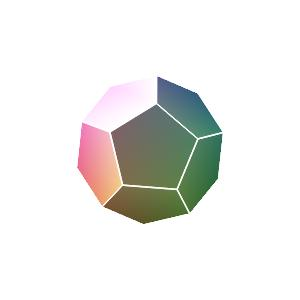
\includegraphics[height=5cm]{dodecahedron.jpg}
%     \caption{正十二面体}\label{}
%\end{minipage} 
%\begin{minipage}{0.4\columnwidth}
%\centering
%     \includegraphics{~/Documents/GitHub/bEuclideanGeo/ch1/images/figureGroup2.9}
%     \caption{正十二面体の模式図}\label{}
%\end{minipage} 
%\end{figure}

\noindent
纏めると以下の表のようになる：
\begin{table}[h]
  \centering
  \begin{tabular}{l|llllllll} 
       \noalign{\hrule height 1pt}
      $G$ &$k$& $\alpha_1$ &$\alpha_2$&$\alpha_3$& $\beta_1$&$\beta_2$&$\beta_3$& $n$ \\ \hline \hline
     $C_n$&2&$n$&$n$&$ $  & $1$&$1$ & $ $& $n$\\ \hline
     $D_m$&3&$2$&$2$&$m$  & $m$&$m$ & $2$& $2m$\\ \hline
     $ T$&3&$2$& $3$ & $3$ &$6$ &$4$ &$4$ & $12$ \\ \hline
     $W$&3& $2$&$3$  & $4$ & $12$&$8$&$6$ &$24$ \\ \hline
     $I$& 3&$2$& $3$ & $5$&$30$ &$20$ &$12$ & $60$\\ \hline
  \noalign{\hrule height 1pt}
\end{tabular}
\caption{$\SO(3)$の有限部分群の分類}
\end{table}

ユークリッドの原論の第13巻にあるように，プラトンの正多面体は

\begin{quote}
正四面体，立方体，正八面体，正一二面体，正二十面体
\end{quote}

\noindent
の$5$種類である．
立方体と正八面体は面と頂点を入れ換える変換で双対であり，正一二面体と正二十面体も双対である．正四面体は自己双対であり，上の表はそれらの像を保つ回転のなす有限部分群の分類に対応していて，
$T$を正四面体群，$Q$を正八面体%（立方体）
群，$I$を正二十面体%（正一二面体）
群という．



%以下の参考文献が%（数理内からアクセスすれば）
%\href{https://link.springer.com/}{ここから}
%ダウンロード可能．
%\begin{thebibliography}{9}
%\item
%L.C.~Grove, C.T~Benson, \textit{Finite reflection groups 2nd Ed.}, GTM99, 1996, Springer
%\end{thebibliography}

%\begin{Quiz}$3$
%$Q$が$S_4$と同形になることを示せ．
%\end{Quiz}
%\begin{Quiz}$4$
%$I$が$A_5$と同形になることを示せ．ただし，$A_5$は5次の交代群である．
%\end{Quiz}


まず，$D_m$が$\Ot(2)$の有限部分群では${}^t(\cos\theta,\sin\theta)$の向きの軸に関する鏡映
\[
     R
     =
     \begin{pmatrix}
          \cos 2\theta &\sin 2\theta\\
          \sin 2\theta&-\cos 2\theta\\
     \end{pmatrix}
\]
から構成されていて，${}^t(\cos\theta,\sin\theta)$が固有値$1$, ${}^t(\sin\theta,-\cos\theta)$が固有値$-1$の固有ベクトルである．
行列$R$の行列式は$-1$である．
$\SO(3)$では
\[
     \tilde R
     =
     \begin{pmatrix}
          \cos 2\theta &\sin 2\theta&0\\
          \sin 2\theta&-\cos 2\theta&0\\
          0&0&-1\\
     \end{pmatrix}
\]
と拡張されていて，
${}^t(\cos\theta,\sin\theta,0)$が固有値$1$, 
${}^t(\sin\theta,-\cos\theta,0)$と ${}^t(0,0,1)$が固有値$-1$の固有ベクトルである．
この行列$\tilde R$の行列式は$1$である．
これは${}^t(\cos\theta,\sin\theta,0)$の向きの軸に関する$\pi$回転である．つまり$2$次元の鏡映は$3$次元の$\pi$回転になることを注意しておく．

表の
$T$を\term[]{正四面体群}(tetrahedron group), $W$を\term[]{正八面体群}(octahedron group)，$I$を\term[]{正二十面体群}(icosahedron group)という．
これらが名前を付けた正多面体の（等長）群に一致することを示すことが出来るが，
時間の節約のため，ここでは正四面体群$T$の場合のみ確かめる：
$\alpha_2=3$のとき$\beta_2=4$なので $\mathbf x_2\in P$が
\[
     G\mathbf x_2
     =
     \{\mathbf y_1, \mathbf y_2,\mathbf y_3,\mathbf y_4\}
     \ni \mathbf x_2
\]
$S\neq E\in \stab(\mathbf x_2)$は$\alpha_2=3$より，$2\pi/3$回転である．回転の極は$\pm \mathbf x_2$なので，全ての
$\mathbf y_i\in G\mathbf x_2$を止めることはない．
$S$の極が$\mathbf y_1$だとすると適当に順番を付け替えて
\[
     S\mathbf y_1=\mathbf y_1,\quad
     S\mathbf y_2=\mathbf y_3,\quad
     S\mathbf y_3=\mathbf y_4,\quad
     S\mathbf y_4=\mathbf y_2
\]
$S$は直交行列なので
\[
\begin{split}
     \|\mathbf y_1-\mathbf y_2\|
     &=
     \|S\mathbf y_1-S\mathbf y_2\|\\
     &=
     \|\mathbf y_1-\mathbf y_3\|
     =
     \|\mathbf y_1-\mathbf y_4\|
\end{split}
\]
$S\in \stab(\mathbf y_2)$, $\stab(\mathbf y_3)$, $\stab(\mathbf y_3)$について同じ議論をすると，$\{\mathbf y_1, \mathbf y_2,\mathbf y_3,\mathbf y_4\}$が正四面体をなすこと，
すべての二点が$G$の元で移りあうこと分かる．
面については，
\[
     \mathbf z_{ijk}=\tfrac13(\mathbf y_i+\mathbf y_j+\mathbf y_k)\quad (i< j<k)
\]
と置けば，最初の$S$については
\[
     S\mathbf z_{234}=\mathbf z_{234}
\]
となるので，$S$は正四面体の頂点と面の重心を通る回転と一致することが分かる．

\begin{figure}[htb]
   \centering
   \begin{minipage}{0.4\columnwidth}
      \centering
       \includegraphics{~/Documents/GitHub/bEuclideanGeo/ch1/images/figureGroup3.1}
       \caption{$2\pi/3$回転}
      \label{}
   \end{minipage} 
   \begin{minipage}{0.4\columnwidth}
      \centering
       \includegraphics{~/Documents/GitHub/bEuclideanGeo/ch1/images/figureGroup3.11}
       \caption{$2\pi/3$回転}
      \label{}
   \end{minipage} 
\end{figure}
\begin{figure}[htb]
   \centering
   \begin{minipage}{0.4\columnwidth}
      \centering
       \includegraphics{~/Documents/GitHub/bEuclideanGeo/ch1/images/figureGroup3.2}
       \caption{$\pi$回転}
   \end{minipage} 
   \begin{minipage}{0.4\columnwidth}
      \centering
       \includegraphics{~/Documents/GitHub/bEuclideanGeo/ch1/images/figureGroup3.12}
       \caption{$\pi$回転}
   \end{minipage} 
\end{figure}

次に$S\neq E\in \stab(\mathbf x_1)$は$\alpha_1=2$より，$\pi$回転である．$G\mathbf x_2$に$S$を作用させて$S\mathbf y_i=\mathbf y_i$とすると，$S\in \stab(\mathbf x_2)$となり，$2\pi/3$回転となり矛盾．よって
\[
     S\mathbf y_i\neq \mathbf y_i
\]
$SS=E$なので，適当に名前を付け替えると
\[
     S\mathbf y_1=\mathbf y_2,\quad
     S\mathbf y_2=\mathbf y_1,\quad
     S\mathbf y_3=\mathbf y_4,\quad
     S\mathbf y_4=\mathbf y_3
\]
したがって
\[
     \mathbf z_{ij}=\tfrac12(\mathbf y_i+\mathbf y_j)\quad (i< j)
\]
と置くと
\begin{gather*}
     S\mathbf z_{12}=\mathbf z_{12},\quad 
     S\mathbf z_{34}=\mathbf z_{34},\\
     S\mathbf z_{13}=\mathbf z_{24},\quad 
     S\mathbf z_{14}=\mathbf z_{23},\quad
     S\mathbf z_{23}=\mathbf z_{14},\quad 
     S\mathbf z_{24}=\mathbf z_{13}
\end{gather*}
となり，正四面体の辺の変換と一致することが分かり，$G=T$が分かる．ただし，ここで等しいとは四頂点の配置分の自由度を除いて等しいということである．

%\begin{Quiz}$3$
%表~\ref{k=3}
%の$D_m$場合も正二面体群$D_m$に一致することを示せ．
%\end{Quiz}
\begin{Quiz}
   表~\ref{classification}
   の$W$の場合も正八面体群$W$に一致することを示せ．
\end{Quiz}
\begin{Quiz}
   表~\ref{classification}
   の$I$の場合も正二十面体群$I$に一致することを示せ．
\end{Quiz}
\begin{Quiz}
   $n$次交代群\footnote{$S_n$の偶置換全体のなす群，補足に詳しい説明を与えてある}を $A_n$と書く．
   正四面体群$T$が$4$次交代群$A_4$と同形になることを示せ．
\end{Quiz}
\begin{Quiz}
   正八面体群
   $W$が$4$次対称群$S_4$と同形になることを示せ．
\end{Quiz}

\begin{Quiz}
   正二十面体群
   $I$が$5$次交代群$A_5$と同形になることを示せ．
\end{Quiz}


\subsection{$3$次直交群の有限部分群}
\begin{Thm}
   $S\in \Ot(3)$が$|S|=-1$をみたすとき，$S$ はある平面についての鏡映
   と，それに直交する軸についての回転になる．
\end{Thm}
\begin{proof}
   Euler の定理の証明とほぼ同じ．
   \begin{figure}[htb]
      \centering
      \begin{minipage}{0.4\columnwidth}
         \centering
         \includegraphics{~/Documents/GitHub/bEuclideanGeo/ch1/images/figureGroup3.3}
         \caption{鏡映と回転}
      \end{minipage} 
      \begin{minipage}{0.4\columnwidth}
         \centering
         \includegraphics{~/Documents/GitHub/bEuclideanGeo/ch1/images/figureGroup3.5}
         \caption{$Z$}\label{Z}
   \end{minipage} 
   \end{figure}
   
   $S\in \Ot(3)$ の固有多項式
   \[
        g_S(t)
        =
        |tE-S|
        =t^3 + \alpha t^2+ \beta t +\gamma
   \]
   は$3$次の実係数多項式なので必ず一つは実数解$\lambda_1$を持つ．$\lambda\in \mathbf R$を実数の固有値，$\mathbf x\neq \mathbf 0$をその固有ベクトルとすると，
   \[
        (\mathbf x,\mathbf x)
        =(S\mathbf x,S\mathbf x)
        =
        (\lambda\mathbf x,\lambda\mathbf x)
        =
        \lambda^2(\mathbf x,\mathbf x)
   \]
   $(\mathbf x,\mathbf x)>0$なので
   $\lambda^2=1$，つまり，
   \[
        \lambda=\pm1
   \]
   が分かる．
   
   $\lambda_2$, $\lambda_3\in \mathbf C$を他の固有値とする．
   $\lambda_2$が実数ならば$\lambda_3$も実数で，
   \[
        |S|=-g_S(0)=\lambda_1\lambda_2\lambda_3
   \]
   $|S|=-1$なので$\lambda_1\lambda_2\lambda_3=-1$となり，
   適当に順番を入れ換えると
   \begin{equation}\label{specialCase}
        \lambda_1=-1, \lambda_2=\lambda_3=1,\quad
        \text{あるいは}\quad
        \lambda_1=\lambda_2=\lambda_1=-1 \tag{*}
   \end{equation}
   のいずれか．
   
   $\lambda_2$が実数でないならば$\lambda_3$はその共役複素数
   となり，全ての固有値が相異なるので，複素正則行列で対角化出来て
   \[
        -1 = |S|=\lambda_1\lambda_2\bar \lambda_2
   \]
   $\lambda_2\bar \lambda_2>0$より$\lambda_1=-1$, $\lambda_2\bar \lambda_2=1$が分かる．
   
   \emptyline
   固有値$-1$の固有ベクトルを$\mathbf x\neq\mathbf 0 $と置く．
   $\mathbf y\in\mathbf R^3$が$(\mathbf y,\mathbf x)=0$を満たすとすると
   \[
        (S\mathbf y,\mathbf x)
        =
        (S\mathbf y,-S\mathbf x)
        =
        -(\mathbf y,\mathbf x)
        =
        0
   \]
   となり，$S$は平面$T=\{\mathbf y\mid (\mathbf y,\mathbf x)=0\}$を保つことが分かる．$S|_T$は$2$次元直交群の元だが，$T$をユークリッド平面と同一視して
   \[
        \det S|_T=
        \begin{cases}
             \lambda_2\bar \lambda_2=1& \lambda_2\notin \mathbf R\\
             (\pm1)^2=1  & \lambda_2,\lambda_3  \text{ is }
                \eqref{specialCase}
        \end{cases}
   \]
   なので，$T$は原点を通り$\mathbf x$を通る直線を軸とする回転になる．つまり
   \[
        S(\xi \mathbf x+ \eta \mathbf y)
        = -\xi \mathbf x+ \eta S_{\theta}\mathbf y
   \]
   ただし，$S_{\theta}$は$ \mathbf x$を中心にした$\theta$回転．
\end{proof}
\eqref{specialCase}の最初のケースは, $\mathbf x$についての単なる($0$回転の)鏡映で，
最後の場合に対応する行列は
\[
     Z=
     \begin{pmatrix}
          -1&0&0\\
          0&-1&0\\
          0&0&-1\\
     \end{pmatrix}
     =-E\in \Ot(3)
\]
である(図~\ref{Z})．つまり，固有空間が$\mathbf R^3$で全ての$\mathbf x\neq \mathbf 0$が固有値$-1$の固有ベクトルである．
また，任意の$R\in \Ot(3)$の元に対して
\[
     ZR = -R = RZ
\]
つまり，$Z$は全ての元と可換である．

\begin{Q}
   $\Ot(3)$の有限部分群の分類？
\end{Q}
$G$を$\Ot(3)$の有限部分群とする．$G\subset \SO(3)$の場合は既に求まったので，$R\in G\setminus  \SO(3)$が存在するとし，$H=G\cap \SO(3)$と置く．これは
$G$の部分群である．
\[
     H =\{S_0=E, S_1, \dots , S_{m-1}\}
\]
と置くと，
\[
     G\supset \{E, S_1, \dots , S_{m-1},R,RS_1, \dots , RS_{m-1}\}
\]
であるが，$R'\in G\setminus  \SO(3)$とすると
\[
     |R^{-1}R'|=|R^{-1}||R'|=(-1)(-1)=1
\]
なので$R^{-1}R'\in H$となり，ある$S_i\in H$が存在して
\[
     R^{-1}R'=S_i\quad\Rightarrow\quad R'=RS_i
\]
よって等号
\begin{equation}\label{G}
     G= \{E, S_1, \dots , S_{m-1},R,RS_1, \dots , RS_{m-1}\}
\end{equation}
が示せた．
\emptyline

case 1) : $Z\in G$のとき$R=Z$として
\[
     G= \{E, S_1, \dots , S_{m-1},Z,ZS_1, \dots , ZS_{m-1}\}
     =:\bar H
\]
と表す．つまり，$G$は$H$に$Z$を加えた群$\bar H$になる．
\emptyline

case 2) : $Z\notin G$のとき
\eqref{G}より
\[
     G^{+}:= \{E, S_1, \dots , S_{m-1},ZRS_0, \dots , ZRS_{m-1}\}
\]
と表すと，$|ZRS_i|=|Z||R||S_1|=-1\times(-1)\times 1=1$より，
$\SO(3)$の有限部分群で$H$を部分群として含むものである．
\[
     (ZRS_i)^{-1}H(ZRS_i)=H,\quad S_i^{-1}HS_i=H
\]
より，指数$2$の正規部分群であり，$H\lhd G^{+}$と表す．

逆に$K$が$\SO(3)$の有限部分群で，その指数$2$の正規部分群$H$を持つとする．
\[
     H=\{E, S_1, \dots , S_{m-1}\},\quad
     K=\{E, S_1, \dots , S_{m-1},T_{0},\dots, T_{m-1}\}
\]
と表すとき
\[     
     K]H:= \{E, S_1, \dots , S_{m-1},ZT_{0},\dots, ZT_{m-1}\}
\]
と置くと$\SO(3)$に含まれない$\Ot(3)$の有限部分群が得られる．

\emptyline

$|K|=2|H|$であることなどに注意して，$\SO(3)$の有限部分群の分類
（表 \ref{classification}）
を見ると，
指数$2$の正規部分群をもつ$\SO(3)$の有限部分群の分類が分かる：
\[
     C_m \lhd C_{2m},\quad C_m\lhd  D_m,\quad 
     D_m \lhd D_{2m},\quad T\lhd W
\]


以上を纏めると：

\begin{Thm}
   $\Ot(3)$の有限部分群は以下のいずれか：
   \begin{enumerate}
      \item
      \[
           C_m,\quad D_m,\quad  T,\quad W,\quad  I
      \]
      
      \item
      \[
           \bar C_m,\quad \bar D_m,\quad, \bar T \quad \bar W, \quad  \bar I
      \]

      \item
      \[
           C_{2m}]C_m,\quad D_m]C_m,\quad D_{2m}]D_m,\quad W]T
      \]
   \end{enumerate}
\end{Thm}
\begin{figure}[htb]
   \centering
   \begin{minipage}{0.4\columnwidth}
      \centering
      \includegraphics{~/Documents/GitHub/bEuclideanGeo/ch1/images/figureGroup3.6}
      \caption{$D_3\lhd D_6$}\label{$D_3D_6$}
   \end{minipage} 
   \begin{minipage}{0.4\columnwidth}
      \centering
      \includegraphics{~/Documents/GitHub/bEuclideanGeo/ch1/images/figureGroup3.4}
      \caption{$T\lhd W$}\label{$TW$}
   \end{minipage} 
\end{figure}
\begin{Quiz}
$\SO(3)$の群$K$とその指数$2$の正規部分$H$群の組が上で上げたものに以外にないことを示し，上で上げたものが確かに指数$2$の正規部分群であることを示せ（図 \ref{$D_3D_6$}, \ref{$TW$} も参考にせよ）．
\end{Quiz}


%以下の\cite{GB}が%（数理内からアクセスすれば）
%\href{https://link.springer.com/}{ここから}
%ダウンロード可能．
%
%\emptyline
%次回から平面結晶群の分類に入る．
%
%\begin{thebibliography}{9}
%   \bibitem{GB}
%   L.C.~Grove, C.T~Benson, \textit{Finite reflection groups 2nd Ed.}, GTM99, 1996, Springer
%\end{thebibliography}



\section{$\SO(3)$の幾つかの有限部分群の構造}
$\SO(3)$の有限部分群と置換群・交代群の関係を調べる．
置換群・交代群については

正二面体群$D_3$が$3$次対称群$S_3$と同形になること：
正三角形の頂点を$1$, $2$, $3$と呼ぶことにする．
$\sigma\in D_3$は頂点を頂点に移すので，頂点$1$ が頂点$i_1$に移り，
頂点$2$ が頂点$i_2$に移り，頂点$3$ が頂点$i_3$に移るとすると
\[
     D_3\ni \sigma\mapsto 
     \begin{pmatrix}1&2&3\\i_1&i_2&i_3\end{pmatrix}\in S_3
\]
で写像が定まる．\eqref{S3}の任意の$S_3$の置換に対応する正三角形の等長変換が存在する．つまり，
二つの$2\pi/3$回転$\begin{pmatrix}1&2&3\end{pmatrix}$, 
$\begin{pmatrix}3&2&1\end{pmatrix}$と単位元が偶置換で，
それら全体は$C_3$と同形となる．
奇置換$\begin{pmatrix}1&2\end{pmatrix}$, $\begin{pmatrix}2&3\end{pmatrix}$, $\begin{pmatrix}3&1\end{pmatrix}$ が$\pi$回転となっていて，単位元とそれぞれの元が$C_2$と同形な$3$つの部分群となっている．
$|S_3|=|D_3|=6$より全単射になる．等長変換の合成は頂点の変換の合成となるので準同形であることも明か．
表~\ref{again}の$D_3$の場合$\pi$回転の$3$個の軸が表の（異なる二つの$G$軌道の）$3+3=6$個の極に対応し，$2\pi/3$回転の$1$個の軸が表の（図では表現できていないが中心の点の上下にある，一つの$G$軌道の）$2$個の極に対応することが確認が出来る．
\begin{table}[h]
     \centering
     \begin{tabular}{l|lllllll} 
          \noalign{\hrule height 1pt}
          $G$ & $\alpha_1$ &$\alpha_2$&$\alpha_3$& $\beta_1$&$\beta_2$&$\beta_3$& $n$ \\ \hline \hline
          $C_m$&$m$ &$m$& &1 &1  & & $m$\\ \hline
          $D_m$&$2$&$2$&$m$  & $m$&$m$ & $2$& $2m$\\ \hline
          $ T$&$2$& $3$ & $3$ &$6$ &$4$ &$4$ & $12$ \\ \hline
          $W$& $2$&$3$  & $4$ & $12$&$8$&$6$ &$24$ \\ \hline
          $I$& $2$& $3$ & $5$&$30$ &$20$ &$12$ & $60$\\ \hline
      \noalign{\hrule height 1pt}
   \end{tabular}
   \caption{$\SO(3)$の有限部分群の分類(再掲)}\label{again}
\end{table}

\begin{figure}[hb]
   \centering
   \begin{minipage}{0.4\columnwidth}
      \centering
        \includegraphics{~/Documents/GitHub/bEuclideanGeo/ch1/images/figureGroup3.131}
        \caption{$3$本の$\pi$回転の軸}\label{quadPi}
   \end{minipage} 
   \begin{minipage}{0.4\columnwidth}
      \centering
        \includegraphics{~/Documents/GitHub/bEuclideanGeo/ch1/images/figureGroup3.13}
        \caption{$4$本の$2\pi/3$回転の軸}\label{quad2Pi/3}
   \end{minipage} 
\end{figure}

正四面体群$T$が$4$次交代群$A_4$と同形であること：
正四面体の頂点を$1$, $2$, $3$, $4$と呼ぶことにする．
表 \ref{again} によれば$\alpha_1=2$のときは三本の軸の回りの$\pi$回転で図 \ref{quadPi}のように
\[
     \begin{pmatrix}1&2\end{pmatrix}
     \begin{pmatrix}3&4\end{pmatrix}, \quad
     \begin{pmatrix}1&3\end{pmatrix}
     \begin{pmatrix}2&4\end{pmatrix}, \quad
     \begin{pmatrix}1&4\end{pmatrix}
     \begin{pmatrix}2&3\end{pmatrix}
\]
の三つの偶置換からなる．これに単位元を付け加えたのがクライン群である．
図 \ref{quad2Pi/3}のように
4本の軸の回りの$\pm 2\pi/3$回転なので$2\times 4=8$個の偶置換
\[
\begin{split}
     &\begin{pmatrix} 2& 3&  4\end{pmatrix},\quad
     \begin{pmatrix} 1& 3&  4\end{pmatrix},\quad
     \begin{pmatrix} 1& 2&  4\end{pmatrix},\quad
     \begin{pmatrix} 1& 2&  3\end{pmatrix},\\
     &\begin{pmatrix} 4& 3&  2\end{pmatrix},\quad
     \begin{pmatrix} 4& 3&  1\end{pmatrix},\quad
     \begin{pmatrix} 4& 2&  1\end{pmatrix},\quad
     \begin{pmatrix} 3& 2&  1\end{pmatrix}
\end{split}
\]
からなるので，$T$の群の位数は$ 1 + 3 +8 = 12$となる．$A_4$は$12$個からなるので$T$から$A_4$への同型が得られる．

\begin{figure}[hb]
   \centering
   \begin{minipage}{0.4\columnwidth}
      \centering
        \includegraphics{~/Documents/GitHub/bEuclideanGeo/ch1/images/figureGroup3.21}
     \caption{正八面体と立方体}\label{octaQube}
   \end{minipage} 
   \begin{minipage}{0.4\columnwidth}
      \centering
        \includegraphics{~/Documents/GitHub/bEuclideanGeo/ch1/images/figureGroup3.22}
        \caption{立方体と正八面体}\label{qubeOcta}
   \end{minipage} 
\end{figure}


正八面体群$W$が$4$次対称群$S_4$と同形になること：
立方体と正八面体はそれぞれの面を点に取換えることで得られるので互いに双対である（図~\ref{octaQube}, \ref{qubeOcta}）ので立方体を使って考える．
図 \ref{cubePi/2} のように正四面体を立方体に埋め込み，
正四面体の頂点を上と同様に$1$, $2$, $3$, $4$と名付ける．
更に残りの頂点には$1$と重心を通る直線が通るもう一つの頂点を同じ$1$と名付けようにして$1$, $2$, $3$, $4$と名付ける．
そして，$1$と命名された$2$つの頂点の集合を$\bar 1$のように表し，
集合$\{\bar 1, \bar 2 ,\bar 3 ,\bar 4\}$の置換と$W$の元が同一視されることを以下で確かめる．
図 \ref{cube2Pi/3}を見ると
例えば$1$と$1$を結ぶ直線を軸にする$\pm 2\pi/3$回転は$1$を止めるので
\[
\begin{split}
     &\begin{pmatrix}\bar 2&\bar 3&  \bar 4\end{pmatrix},\quad
     \begin{pmatrix} \bar 1& \bar 3&  \bar 4\end{pmatrix},\quad
     \begin{pmatrix} \bar 1& \bar 2&  \bar 4\end{pmatrix},\quad
     \begin{pmatrix} \bar 1& \bar 2&  \bar 3\end{pmatrix},\\
     &\begin{pmatrix} \bar 4& \bar 3&  \bar 2\end{pmatrix},\quad
     \begin{pmatrix} \bar 4& \bar 3&  \bar 1\end{pmatrix},\quad
     \begin{pmatrix} \bar 4& \bar 2&  \bar 1\end{pmatrix},\quad
     \begin{pmatrix} \bar 3& \bar 2&  \bar 1\end{pmatrix}
\end{split}
\]
の$8$個の三換（偶置換）からなる．
図 \ref{cubePi/2} を見ると$\pi/2$回転から生成され
その回転軸が三本あり，そのうちの半数が正四面体を固定する$\pi$回転$3$個であり，置換としては
\[
     \begin{pmatrix}\bar 1&\bar 2\end{pmatrix}
     \begin{pmatrix}\bar 3&\bar 4\end{pmatrix},\quad
     \begin{pmatrix}\bar 1&\bar 3\end{pmatrix}
     \begin{pmatrix}\bar 2&\bar 4\end{pmatrix},\quad
     \begin{pmatrix}\bar 1&\bar 4\end{pmatrix}
     \begin{pmatrix}\bar 2&\bar 3\end{pmatrix}
\]
である．これらに恒等写像を加えた$8+3+1=12$個の偶置換全体が正四面体を固定する等長群をなし，$A_4$と同型である．
さらに正四面体を固定しない$\pi/2$回転は
\[
\begin{split}
     &\begin{pmatrix}\bar 1&\bar 2&\bar 3&\bar 4\end{pmatrix},\quad
     \begin{pmatrix}\bar 4&\bar 3&\bar 2&\bar 1\end{pmatrix},\quad
     \begin{pmatrix}\bar 1&\bar 2&\bar 4&\bar 3\end{pmatrix},\\
     &\begin{pmatrix}\bar 3&\bar 4&\bar 2&\bar 1\end{pmatrix},\quad
     \begin{pmatrix}\bar 1&\bar 3&\bar 2&\bar 4\end{pmatrix},\quad
     \begin{pmatrix}\bar 4&\bar 2&\bar 3&\bar 1\end{pmatrix}
\end{split}
\]
という$6$個の長さ$4$の循環置換からなる奇置換である．
\begin{figure}[th]
   \centering
   \begin{minipage}{0.4\columnwidth}
      \centering
        \includegraphics{~/Documents/GitHub/bEuclideanGeo/ch1/images/figureGroup3.15}
        \caption{$4$本の$2\pi/3$回転の軸}\label{cube2Pi/3}
   \end{minipage} 
   \begin{minipage}{0.4\columnwidth}
      \centering
        \includegraphics{~/Documents/GitHub/bEuclideanGeo/ch1/images/figureGroup3.14}
        \caption{$3$本の$\frac{\pi}{2}$回転の軸} \label{cubePi/2}
      \label{}
   \end{minipage} 
\end{figure}

図 \ref{cubePi} の$\pi$回転は
$\begin{pmatrix}
      4\\2
\end{pmatrix}
= 6$ 個の奇置換(互換)
$\begin{pmatrix}\bar i&\bar j\end{pmatrix}$($i\neq j$)を成している．
言い換えると$S_4$の奇置換全体$12$個を含んでいて，
$W$から$S_4$への同型写像が得られた．

\begin{figure}[hb]
   \centering
   \begin{minipage}{0.4\columnwidth}
   \centering
        \includegraphics{~/Documents/GitHub/bEuclideanGeo/ch1/images/figureGroup3.16}
        \caption{$6$本の$\pi$回転の軸}\label{cubePi}
   \end{minipage} 
   \begin{minipage}{0.4\columnwidth}
   \centering
        \includegraphics{~/Documents/GitHub/bEuclideanGeo/ch1/images/figureGroup3.18}
        \caption{正二十面体と正十二面体}\label{IcosaDual1}
   \end{minipage} 
\end{figure}
\emptyline


\begin{figure}[hb]
   \centering
   \begin{minipage}{0.4\columnwidth}
      \centering
        \includegraphics{~/Documents/GitHub/bEuclideanGeo/ch1/images/figureGroup3.19}
        \caption{正十二面体と正二十面体}\label{IcosaDual2}
   \end{minipage} 
   \begin{minipage}{0.4\columnwidth}
      \centering
        \includegraphics{~/Documents/GitHub/bEuclideanGeo/ch1/images/figureGroup3.20}
     \caption{正十二面体と立方体}\label{dodecaQube}
   \end{minipage} 
\end{figure}

正二十面体群
$I$が$5$次交代群$A_5$と同形になること：
正十二面体と正二十面体はそれぞれの面を点に取換えることで得られるので互いに双対である（図~\ref{IcosaDual1}, \ref{IcosaDual2}）．
そこで
$I$を正十二面体\footnote{作図へのコメント：$\tau$を黄金比とし$(\pm \tau,\pm \tau,\pm \tau)$を立方体の$8$つの頂点の座標とする．この立方体を含む正十二面体の立方体の頂点でない$20-8=12$個の頂点の座標を$(\pm1, 0, \pm(1+\tau))$, $(\pm(1+\tau), \pm1, 0)$, $(0, \pm(1+\tau), \pm1)$とすると，一辺$2$の正十二面体が描ける．正二十面体はそれらの頂点の重心を取れば良い，}の等長群と見て考察する．まず，正十二面体に立方体
を埋め込むことを考える（図~\ref{dodecaQube}）．立方体の辺は$12$個あり，その全てが正十二面体の$12$個の面の中に一本ずつ入っていることを確認してほしい．
次に，正二十面体の$20$個の頂点に$1, 2, 3, 4, 5$ を$4$個ずつ置く．
ただし，各正五角形は全ての異なる$1, 2, 3, 4, 5$が配置されているものを考える．そのため，まず，図~\ref{nameDodeca}の赤の正五角形に$1, 2, 3, 4, 5$を反時計回りに配置し，それらの頂点と未だ名前のない頂点を含む辺の頂点を$ \mod 5$で$2$を足した数で名付けると，新しい頂点には反時計回りに$1, 2, 3, 4, 5$を配置されていることがわかる．未だ名前が一個だけ足りない各正五角形の頂点には足りない$1, 2, 3, 4, 5$を配置することが出来て，これらの新しい頂点にも反時計回りに$1, 2, 3, 4, 5$が配置されていることもわかる．これらの新しい頂点と未だ名前のない頂点含む辺の頂点に$ \mod 5$で$2$を足した数で名付けると，新しい頂点には反時計回りに$1, 2, 3, 4, 5$を配置している
ことがわかる．これで欲しい頂点の配置が求まった．

\begin{figure}[hb]
   \centering
   \begin{minipage}{0.4\columnwidth}
      \centering
        \includegraphics{~/Documents/GitHub/bEuclideanGeo/ch1/images/figureGroup3.26}
        \caption{正十二面体の頂点名}\label{nameDodeca}
   \end{minipage} 
   \begin{minipage}{0.4\columnwidth}
      \centering
        \includegraphics{~/Documents/GitHub/bEuclideanGeo/ch1/images/figureGroup3.27}
     \caption{$\bar 5$を止める$\pi$回転}\label{piRote}
   \end{minipage} 
\end{figure}

\begin{figure}[hb]
     \centering
        \begin{minipage}{0.4\columnwidth}
        \centering
        \includegraphics{~/Documents/GitHub/bEuclideanGeo/ch1/images/figureGroup3.28}
        \caption{$\bar 5$を止める$\pm2\pi/3$回転}\label{2pi/3Rote}
   \end{minipage} 
     \begin{minipage}{0.4\columnwidth}
           \centering
           %\includegraphics{~/Documents/GitHub/bEuclideanGeo/ch1/images/figureGroup3.23}
          \includegraphics{~/Documents/GitHub/bEuclideanGeo/ch1/images/figureGroup3.25}
           \caption{ $\frac{2\pi}{5}$ 回転と $(1\,2\,3\,4\,5)$}\label{qubes5}
   \end{minipage} 
\end{figure}


$1$と命名された頂点の集合を$\bar 1$のように表し，
集合$\{\bar 1, \bar 2 ,\bar 3 ,\bar 4, \bar 5\}$の偶置換と$I$の元が同一視されることを以下で確かめる．
図~\ref{dodecaQube}の立方体の$8$個の頂点には$5$の頂点が$4$個，
残りに$1, 2, 3, 4$が一個づつ配置されている（図 \ref{piRote}, \ref{2pi/3Rote}）．
$I$の元でこの立方体を動かさないのは図 \ref{piRote}, \ref{2pi/3Rote}に示した$\pi$回転と$\pm2\pi/3$回転であり，$\pi$回転は$\{\bar 1, \bar 2 ,\bar 3 ,\bar 4\}$の独立な互換の積
\[
     \begin{pmatrix}\bar 1&\bar 2\end{pmatrix}
     \begin{pmatrix}\bar 3&\bar 4\end{pmatrix},\quad
     \begin{pmatrix}\bar 1&\bar 4\end{pmatrix}
     \begin{pmatrix}\bar 2&\bar 3\end{pmatrix},\quad
     \begin{pmatrix}\bar 1&\bar 3\end{pmatrix}
     \begin{pmatrix}\bar 2&\bar 4\end{pmatrix}
\]
であり，$\pm 2\pi/3$回転も$\{\bar 1, \bar 2 ,\bar 3 ,\bar 4\}$の（偶置換の）三環
\[
\begin{split}
     &\begin{pmatrix}\bar 2&\bar 3& \bar 4\end{pmatrix},\quad
     \begin{pmatrix}\bar 1&\bar 3& \bar 4\end{pmatrix},\quad
     \begin{pmatrix}\bar 1&\bar 2& \bar 4\end{pmatrix},\quad
     \begin{pmatrix}\bar 1&\bar 2& \bar 3\end{pmatrix},\\
     &\begin{pmatrix}\bar 4&\bar 3& \bar 2\end{pmatrix},\quad
     \begin{pmatrix}\bar 4&\bar 3& \bar 1\end{pmatrix},\quad
     \begin{pmatrix}\bar 4&\bar 2& \bar 1\end{pmatrix},\quad
     \begin{pmatrix}\bar 3&\bar 2& \bar 1\end{pmatrix}
\end{split}
\]
を生成する．これらは全ての頂点の組に矛楯なく作用していることを確かめてほしい．上で述べたようにそれらは正四面体群$T$を成し，
$\bar 5$を動かさない$4$次交代群$A_4$と同形となっている．
%更に正十二面体の中の異なる5つの立方体が取れ（図 \ref{qubes1}, \ref{qubes2}），異なる立方体毎に5つの正四面体群を作っている．


%\begin{figure}[hb]
%   \centering
%   \begin{minipage}{0.4\columnwidth}
%      \centering
%        \includegraphics{~/Documents/GitHub/bEuclideanGeo/ch1/images/figureGroup3.27}
%        \caption{正十二面体と立方体}
%   \end{minipage} 
%   \begin{minipage}{0.4\columnwidth}
%        \centering
%        \includegraphics{~/Documents/GitHub/bEuclideanGeo/ch1/images/figureGroup3.21}
%        \caption{$3$本の$\pi$回転の軸}\label{piRote}
%   \end{minipage} 
%\end{figure}

表 \ref{again}（とEuler の定理）によれば, $I$の合同変換には$\pi$回転と$2\pi/3$回転の他に
正5角形の二つの面を保つ$2\pi/5$回転がある．
特に図~\ref{qubes1}の正5角形を回転する回転の生成元として
\[
     \sigma
     =\begin{pmatrix}\bar 1&\bar 2&\bar 3& \bar 4&\bar 5\end{pmatrix}
\]
が取れる．これも全ての頂点の組に矛楯なく作用していて，偶置換であることもアミダクジの時と同じように示せる．
$\sigma^n$ $(n =1, 2, 3, 4)$によりが図~\ref{dodecaQube}の立方体を別の立方体に置換するかを示したのが図~\ref{qubes1}--\ref{qubes4} である．$n=1, 2, 3, 4, 5$として
$\bar n$を止める立方体を保存する$I$の部分群を$A_4^n$と置くと
$g=\sigma^n$の内部自己同形の作用で
\[
     A_4^5\ni \tau\mapsto  g\tau g^{-1}\in A_4^n\subset A_5
\]
となる．$A_4^5$ は$\bar 5$を止める全ての三環を含んでいるので，$n = 1, 2, 3, 4, 5$を動かすと$A_5$は全ての三環を含んでいることがわかる．
$A_5$が可解でないことを示したところでコメントしたように
$A_5$は三環で生成されるので，
$I$は$A_5$への全射となり，同型になる．

\begin{figure}[thb]
   \begin{minipage}{0.4\columnwidth}
           \centering
           \includegraphics{~/Documents/GitHub/bEuclideanGeo/ch1/images/figureGroup3.29}
           \caption{$\bar 1$を止める立方体}\label{qubes1}
   \end{minipage} 
   \begin{minipage}{0.4\columnwidth}
     \centering
      \includegraphics{~/Documents/GitHub/bEuclideanGeo/ch1/images/figureGroup3.30}
      \caption{$\bar 2$を止める立方体}\label{qubes2}
   \end{minipage} 
\end{figure}

\begin{figure}[t]
   \begin{minipage}{0.4\columnwidth}
     \centering
      \includegraphics{~/Documents/GitHub/bEuclideanGeo/ch1/images/figureGroup3.31}
      \caption{$\bar 3$を止める立方体}\label{qubes3}
   \end{minipage} 
   \begin{minipage}{0.4\columnwidth}
           \centering
           \includegraphics{~/Documents/GitHub/bEuclideanGeo/ch1/images/figureGroup3.32}
           \caption{$\bar 4$を止める立方体}\label{qubes4}
   \end{minipage} 
\end{figure}

他の方法でも$I$は$A_5$と同型になることを示すことができる．
まず，$60$個の$I$の元のうち
三環は$5$個から$3$個の数字を選ぶことに対応するので
$\begin{pmatrix}
     5\\
     3
\end{pmatrix}
=10$種類あり，
それらはそれぞれ$3$次循環群をなすので，三環は合計$10\times (3-1)=20$個ある．
独立な互換の積は$5$個の数字から$1$個除き，
残りの$4$個の数字を$3$種のペアに分けることに対応するので合計
$5\times 3=15$個ある．
ここから更に単位元（偶置換）$1$個をそぞいた$60-36=24$個が残っている．
そこで$\bar 1, \bar 2 ,\bar 3 ,\bar 4, \bar 5$の長さ$5$の循環置換（これは偶置換である）を考える．
これらは$5!$個ありそうだが$\begin{pmatrix}\bar 1&\bar 2&\bar 3& \bar 4&\bar 5\end{pmatrix}$と$\begin{pmatrix}\bar 3& \bar 4&\bar 5&\bar 1&\bar 2\end{pmatrix}$
は同じ置換を表しているので$5!/5=4!=24$個ある．
そこで図 \ref{nameDodeca}の$12$ある面のうち
表の$6$個の面の頂点の配置を反時計向きに$1$から始まるように並べると，異なる
長さ$5$の循環置換
\[
\begin{split}
     &\begin{pmatrix}\bar 1&\bar 2&\bar 3&\bar 4&\bar 5\end{pmatrix},\quad
     \begin{pmatrix}\bar 1&\bar 3&\bar 5&\bar 4&\bar 2\end{pmatrix},\quad
     \begin{pmatrix}\bar 1&\bar 5&\bar 3&\bar 2&\bar 4\end{pmatrix},\\
     &\begin{pmatrix}\bar 1&\bar 4&\bar 3&\bar 5&\bar 2\end{pmatrix},\quad
     \begin{pmatrix}\bar 1&\bar 3&\bar 2&\bar 5&\bar 4\end{pmatrix},\quad
     \begin{pmatrix}\bar 1&\bar 5&\bar 2&\bar 4&\bar 3\end{pmatrix}
\end{split}
\]
が見つかる，これらはそれぞれ$I$の$2\pi/5$の回転であり，それらは$5$次の巡回群を生成している．
各面の（一番遠い）反対側の面が逆の循環置換になっていることもチェック出来る．
これらの生成する長さ$5$の循環置換の個数は$6\times(5-1)=24$個（表 \ref{5cyclic}）であり，
これらが残りの$24$個の偶置換となっている．
このことから$I$は$A_5$と同型になることが分かる．
\begin{table}[h]
     \centering
     \begin{tabular}{l|lll} 
          \noalign{\hrule height 1pt}
          $\tau$ 
          & $\begin{pmatrix}\bar 1&\bar 2&\bar 3&\bar 4&\bar 5\end{pmatrix}$ 
          &$\begin{pmatrix}\bar 1&\bar 3&\bar 5&\bar 4&\bar 2\end{pmatrix}$
          &$\begin{pmatrix}\bar 1&\bar 5&\bar 3&\bar 2&\bar 4\end{pmatrix}$ \\ 
          $\tau^2$ 
          & $\begin{pmatrix}\bar 1&\bar 3&\bar 5&\bar 2&\bar 4\end{pmatrix}$ 
          &$\begin{pmatrix}\bar 1&\bar 5&\bar 2&\bar 3&\bar 4\end{pmatrix}$
          &$\begin{pmatrix}\bar 1&\bar 3&\bar 4&\bar 5&\bar 2\end{pmatrix}$ \\ 
          $\tau^3$ 
          & $\begin{pmatrix}\bar 1&\bar 4&\bar 2&\bar 5&\bar 3\end{pmatrix}$ 
          &$\begin{pmatrix}\bar 1&\bar 4&\bar 3&\bar 2&\bar 5\end{pmatrix}$
          &$\begin{pmatrix}\bar 1&\bar 2&\bar 5&\bar 4&\bar 3\end{pmatrix}$ \\   
          $\tau^4$ 
          & $\begin{pmatrix}\bar 1&\bar 5&\bar 4&\bar 3&\bar 2\end{pmatrix}$ 
          &$\begin{pmatrix}\bar 1&\bar 2&\bar 4&\bar 5&\bar 3\end{pmatrix}$
          &$\begin{pmatrix}\bar 1&\bar 4&\bar 2&\bar 3&\bar 5\end{pmatrix}$ \\  
          $\tau^5$ 
          & $\qquad\quad\varepsilon$  &  $\qquad\quad\varepsilon$ & 
               $\qquad\quad\varepsilon$  \\
          \noalign{\hrule height 1pt}
   \end{tabular}
\end{table}

\begin{table}[h]
     \centering
   \begin{tabular}{l|lll} 
          \noalign{\hrule height 1pt}
          $\tau$ 
          &$\begin{pmatrix}\bar 1&\bar 4&\bar 3&\bar 5&\bar 2\end{pmatrix}$ 
          &$\begin{pmatrix}\bar 1&\bar 3&\bar 2&\bar 5&\bar 4\end{pmatrix}$
          &$\begin{pmatrix}\bar 1&\bar 5&\bar 2&\bar 4&\bar 3\end{pmatrix}$ \\ 
          $\tau^2$ 
          & $\begin{pmatrix}\bar 1&\bar 3&\bar 2&\bar 4&\bar 5\end{pmatrix}$ 
          &$\begin{pmatrix}\bar 1&\bar 2&\bar 4&\bar 3&\bar 5\end{pmatrix}$
          &$\begin{pmatrix}\bar 1&\bar 2&\bar 3&\bar 5&\bar 4\end{pmatrix}$ \\ 
          $\tau^3$ 
          &$\begin{pmatrix}\bar 1&\bar 5&\bar 4&\bar 2&\bar 3\end{pmatrix}$ 
          &$\begin{pmatrix}\bar 1&\bar 5&\bar 3&\bar 4&\bar 2\end{pmatrix}$
          &$\begin{pmatrix}\bar 1&\bar 4&\bar 5&\bar 3&\bar 2\end{pmatrix}$ \\   
          $\tau^4$ 
          &$\begin{pmatrix}\bar 1&\bar 2&\bar 5&\bar 3&\bar 4\end{pmatrix}$ 
          &$\begin{pmatrix}\bar 1&\bar 4&\bar 5&\bar 2&\bar 3\end{pmatrix}$
          &$\begin{pmatrix}\bar 1&\bar 3&\bar 4&\bar 2&\bar 5\end{pmatrix}$ \\  
          $\tau^5$ 
          &$\qquad\quad\varepsilon$  &  $\qquad\quad\varepsilon$ & 
               $\qquad\quad\varepsilon$  \\
          \noalign{\hrule height 1pt}
   \end{tabular}
   \caption{24個の長さ5の巡回置換}\label{5cyclic}
\end{table}


%\newpage

%\end{document}


